%!TEX root = ../StatisticalCorrelations.tex

\graphicspath{{Body/Figures/EvW/}}

\section{Monte Carlo}


In order to determine correlation coefficients between the various analyses, a Monte Carlo simulation was developed. This Monte Carlo generates pseudo-data according to the different analysis types, fills histograms defined by the parameters in \tabref{tab:analyzerParameters}, and then fits them accordingly. Pseudo-data was generated using \ROOT's \texttt{TF2->GetRandom2()} method. The 2D function used to generate the data is given by a five parameter function with energy dependence on the number, asymmetry, and phase terms,
\begin{align}
	N(t, E) = N_{0}(E) \cdot e^{-t/\tau_{\mu}} \cdot (1 + A(E) \cos{(\omega_{a}t + \phi(E))}),
\label{eq:2dfunc}
\end{align}
with the time-dilated muon lifetime \taumu equal to \ns{64440} and \gmtwo frequency \wa set as
\begin{align}
	\omega_{a} = 2\pi \cdot 0.2291 \text{MHz} \cdot (1 + R \times 10^{-6}),
\end{align}
where \R was set to 0. 


The energy dependent terms in \equref{eq:2dfunc} were determined from energy-binned fits to the data provided by D. Sweigart for ReconEast and M. Sorbara for ReconWest, for each of the four datasets in \Rone. \figref{fig:energyBinFits} show the respective histograms for the 9d dataset, where it can be seen that energy bin fits to the two reconstructions produce very similar histograms. The \RE energy bin fits ranged from \SIrange{300}{3100}{\MeV} in bins of \SI{50}{\MeV} for a total of 56 energy bins, while the \RW energy bin fits ranged from \SIrange{300}{3060}{\MeV} in bins of \SI{60}{\MeV} for a total of 46 energy bins. Two \texttt{TF2}s were constructed using either the \RE or \RW histograms as input. The number of Y points in the functions were set as the number of bins in the respective histograms, and the function was defined such that the energy binned histograms would be linearly interpolated between the values at the bin centers. The number of X points in the functions were defined such that the function ranged from \SIrange{0}{699971.8}{ns} in steps of $149.2/2 = 74.6 \text{ns}$ for a total of 9383 points. This `point-width' was chosen for a couple of reasons. The first is that the maximum number of allowed X or Y points in a \texttt{TF2} is 10000, and this point-width results in a number of points close to but not above that value. The second is that it is either exactly or very close to a multiple of the bin widths chosen by the analyzers. It was found that using the maximum number of points such that the point width was \ns{70} (for a range up to \ns{700000}) resulted in aliasing frequencies appearing in the generated data. With a point-width of \ns{74.6} these aliasing frequencies disappeared entirely except in some Q-Method fits, as evidenced by the non-flat p-value distribution in \figref{}. In order to remove this issue entirely a different implementation beyond \texttt{TF2} would be needed. The 2D function parameters are summarized in \tabref{tab:2dfunctionParameters}.



\begin{figure}[]
\centering
    \begin{subfigure}[t]{0.45\textwidth}
        \centering
        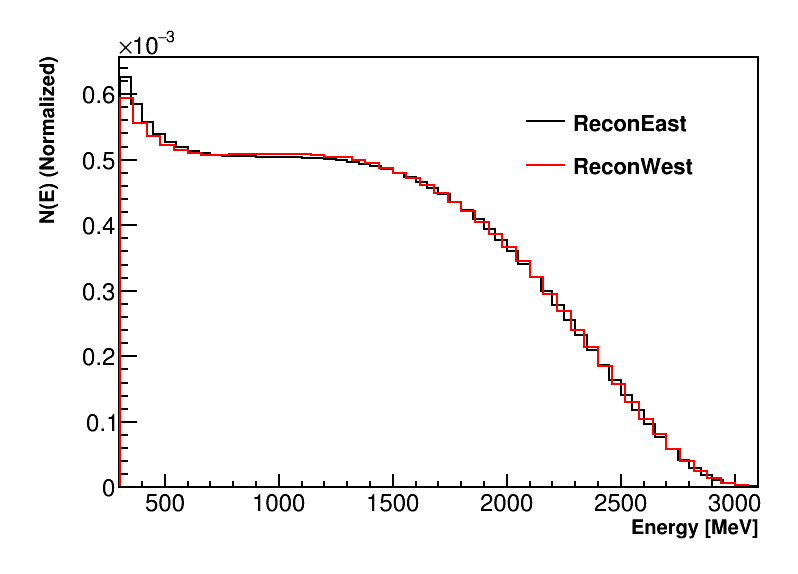
\includegraphics[width=\textwidth]{ReconEastvWest_N}
        \caption{$N(E)$}
    \end{subfigure}% %you need this % here to add spacing between subfigures

    \begin{subfigure}[t]{0.45\textwidth}
        \centering
        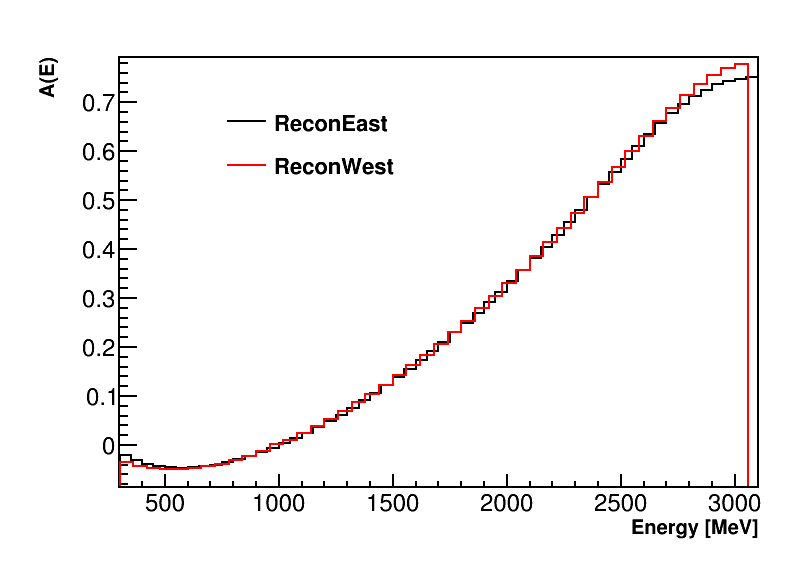
\includegraphics[width=\textwidth]{ReconEastvWest_A}
        \caption{$A(E)$}
    \end{subfigure}
    \hspace{1mm}
    \begin{subfigure}[t]{0.45\textwidth}
        \centering
        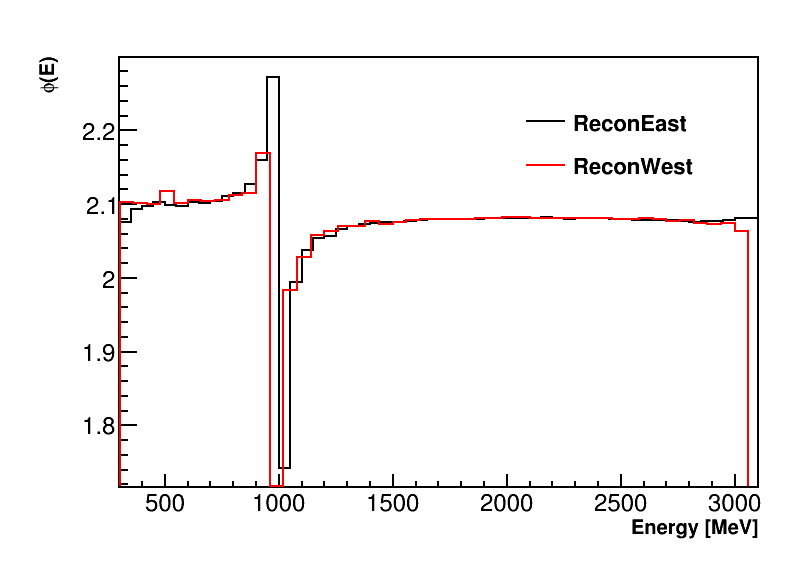
\includegraphics[width=\textwidth]{ReconEastvWest_Phi}
        \caption{$\phi(E)$}
    \end{subfigure}
\caption[]{$N$, $A$, and $\phi$ as a function of energy from energy bin fits to \RE (black) and \RW (red) data for the 9d dataset. These histograms are representative of the quantities for all datasets, though there are slight differences. The \RE energy bin fits ranged from \SIrange{300}{3100}{\MeV} in bins of \SI{50}{\MeV} for a total of 56 energy bins, while the \RW energy bin fits ranged from \SIrange{300}{3060}{\MeV} in bins of \SI{60}{\MeV} for a total of 46 energy bins, hence the different bin edges in the plot. There are some slight differences at low and high energies within the various plots, but for the most part the two reconstructions behave very similary.}
\label{fig:energyBinFits}
\end{figure}



\begin{table}
\centering
\renewcommand{\arraystretch}{1.2}
\begin{tabularx}{1\linewidth}{@{\extracolsep{\fill}}lcc}
  \hline
    \multicolumn{3}{c}{\textbf{2D Function Parameters}} \\
  \hline\hline
     & \thead{\RE Input} & \thead{\RW Input} \\
  \hline
  	Energy Range (\MeV) & 300--3100 & 300--3060 \\
  	Energy Points & 56 & 46 \\ 
  	Energy Point-Width (\MeV) & 50 & 60 \\
  	Time Range (ns) & 0--699971.8 & 0--699971.8 \\
  	Time Points & 9383 & 9383 \\
  	Time Point-Width (ns) & 74.6 & 74.6 \\
  \hline
\end{tabularx}
\caption[]{Parameters used to define the \texttt{TF2}s in the Monte Carlo pseudo-data generation.}
\label{tab:2dfunctionParameters}
\end{table}






\begin{figure}[]
\centering
    \begin{subfigure}[t]{0.45\textwidth}
        \centering
        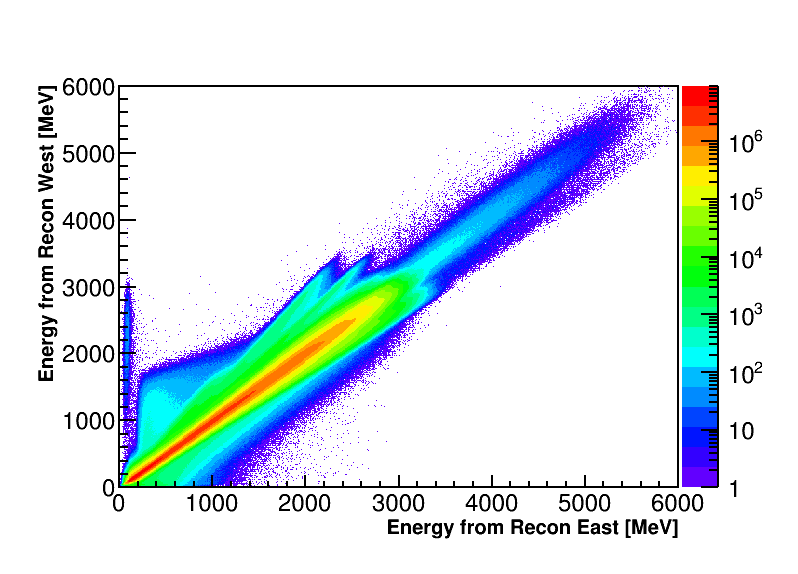
\includegraphics[width=\textwidth]{ReconEastvWest_Energies}
        \caption{}
    \end{subfigure}
    \hspace{1mm}
    \begin{subfigure}[t]{0.45\textwidth}
        \centering
        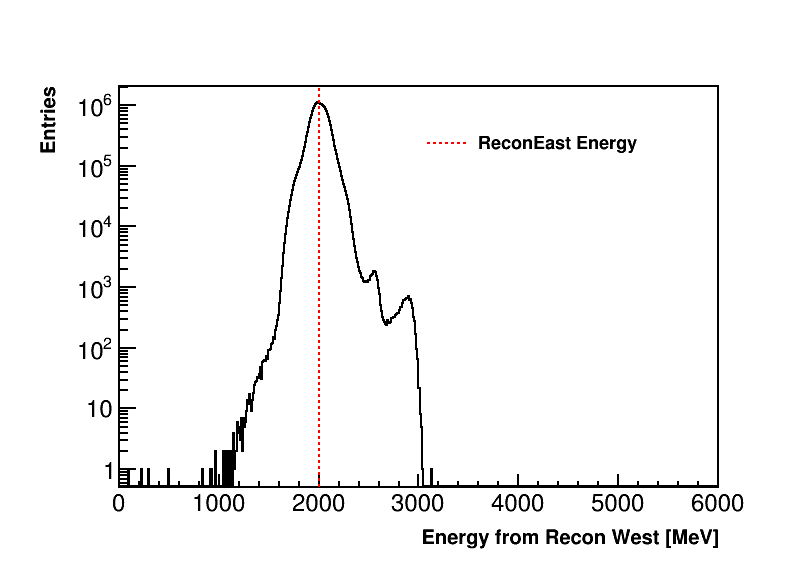
\includegraphics[width=\textwidth]{ReconEastvWest_Projection}
        \caption{}
    \end{subfigure}
\caption[]{Caption}
\label{fig:}
\end{figure}













- don't do pileup, the effect should be a lot smaller than the energy threshold changes between analyses after pileup subtraction, it would be a major effort to somehow put in different pileup cases, etc.

